\subsection{SM4默认XBox查表与XBox合并}
在SM4加密算法的每轮循环中需要对输入的每个字做非线性的过S盒操作,和线性的L操作,
对于
\[ X_3 = a_0||a_1||a_2||a_3  \]
为最后一个32bit分组,分别过S盒后得到
\[ B = b_0 || b_1 |\ b_2 || b_3 = Sbox(a_0)||Sbox(a_1)||Sbox(a_2)||Sbox(a_3)  \]
在代码中通过移位拼接:
\[ B = (b_0 << 24) \oplus (b_1 << 16) \oplus (b_2 << 8) \oplus(b_3) \]
由于L是线性操作,满足
\[  L(a \oplus b) = L(a) \oplus L(b) \]
因此
\begin{equation}
\begin{aligned} 
 L(B)& = L(b_0 << 24) \oplus L(b_1 << 16) \oplus L(b_2 << 8) \oplus L(b_3) \\
     & = B \oplus ROL(B,2) \oplus ROL(B,10) \oplus ROL(B,18) \oplus ROL(24)\\
     & = ROL(Xbox[b_0],24) \oplus ROL(Xbox[b_1],16) \oplus ROL(Xbox[b_2],8) \oplus Xbox[b_3]
\end{aligned}
\end{equation}

\subsubsection{SM4默认XBox查表}
因此预计算$Xbox[i] = L(S(i))$共$2^8 = 256$项,最后循环移位并异或即可得到最终结果。关键代码如下:
\begin{lstlisting}
static void sm4EncryptBlock(const uint32_t rk[32],
                            const uint8_t in[16],
                            uint8_t out[16])
{
    uint32_t X0, X1, X2, X3;
    {
        uint32_t arr[4];
        sm4LoadBlock(in, arr);
        X0 = arr[0]; X1 = arr[1]; X2 = arr[2]; X3 = arr[3];
    }

    initXbox();

    for (int i = 0; i < 32; i++) {
        uint32_t t    = X1 ^ X2 ^ X3 ^ rk[i];
        uint8_t  b0   = (uint8_t)((t >> 24) & 0xFF);
        uint8_t  b1   = (uint8_t)((t >> 16) & 0xFF);
        uint8_t  b2   = (uint8_t)((t >>  8) & 0xFF);
        uint8_t  b3   = (uint8_t)( t        & 0xFF);

        uint32_t newX0 = X0 ^ ROL(xbox[b0], 24)
                            ^ ROL(xbox[b1], 16)
                            ^ ROL(xbox[b2],  8)
                            ^     xbox[b3];

        X0 = X1; X1 = X2; X2 = X3; X3 = newX0;
    }

    {
        uint32_t arr[4] = {X0, X1, X2, X3};
        sm4StoreBlock(arr, out);
    }
}
\end{lstlisting}
编译运行结果截图如下:
\begin{figure}[H]
    \centering
    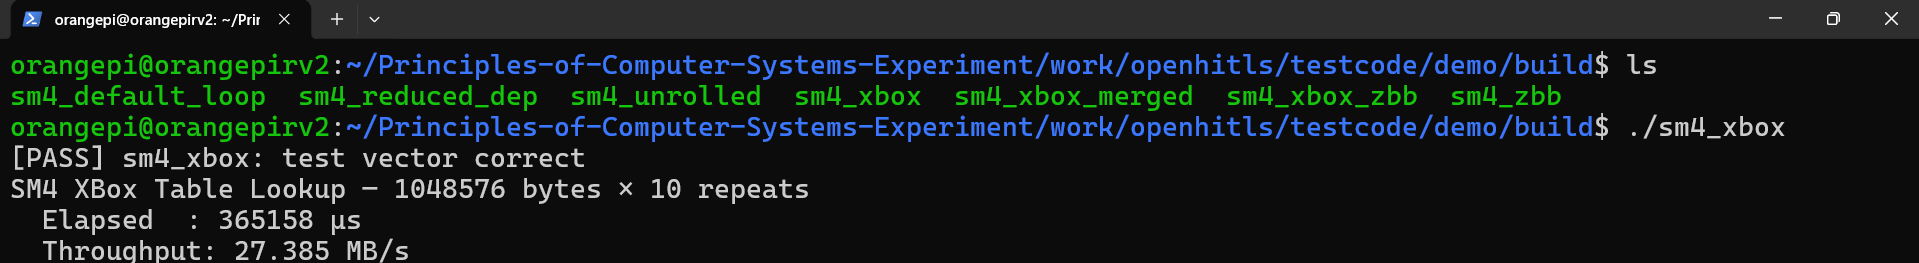
\includegraphics[width = 1\textwidth]{figure/sm4_xbox}
    \caption{SM4默认XBox}
\end{figure}
效率较SM4默认循环和循环展开都有所提升,不过这种提前计算会增大程序的空间复杂度。


\subsubsection{XBox合并}
观察(1)式可以发现最后循环移位的位数是固定的(分别为24、16、8、0),可以分别预计算这里的固定位数循环移位,
将原本运行时计算ROL改为编译时计算且运行时查表,实现Xbox合并。即计算:
\[
\begin{cases}
    XBox0[i] = L(S(i))\\
    XBox1[i] = ROL(L(S(i)),8)\\
    XBox2[i] = ROL(L(S(i)),16)\\
    XBox3[i] = ROL(L(S(i)),24)
\end{cases}
\]
那么实际运行时各个位置查对应的表即可:
\[
\begin{cases}
    ROL(Xbox[b_0],24) = XBox3[b_0]\\
    ROL(Xbox[b_1],16) = XBox2[b_1]\\
    ROL(Xbox[b_2],8) = XBox1[b_2]
\end{cases}
\]
关键代码如下:
\begin{lstlisting}
static uint32_t XBOX0[256];
static uint32_t XBOX1[256];
static uint32_t XBOX2[256];
static uint32_t XBOX3[256];
static int xbox_merged_initialized = 0;

static inline uint32_t ROL(uint32_t x, int n)
{
    return (x << n) | (x >> (32 - n));
}

static void initXboxMerged(void)
{
    if (xbox_merged_initialized) return;

    for (int i = 0; i < 256; i++) {
        XBOX0[i] = sm4L((uint32_t)sm4Sbox((uint8_t)i));
        XBOX1[i] = ROL(XBOX0[i],  8);
        XBOX2[i] = ROL(XBOX0[i], 16);
        XBOX3[i] = ROL(XBOX0[i], 24);
    }
    xbox_merged_initialized = 1;
}

static void sm4EncryptBlock(const uint32_t rk[32],
                            const uint8_t in[16],
                            uint8_t out[16])
{
    uint32_t X0, X1, X2, X3;
    {
        uint32_t arr[4];
        sm4LoadBlock(in, arr);
        X0 = arr[0]; X1 = arr[1]; X2 = arr[2]; X3 = arr[3];
    }

    initXboxMerged();

    for (int i = 0; i < 32; i++) {
        uint32_t t    = X1 ^ X2 ^ X3 ^ rk[i];
        uint32_t newX0 = X0 ^ XBOX3[(t >> 24) & 0xFF]
                           ^ XBOX2[(t >> 16) & 0xFF]
                           ^ XBOX1[(t >>  8) & 0xFF]
                           ^ XBOX0[ t        & 0xFF];

        X0 = X1; X1 = X2; X2 = X3; X3 = newX0;
    }

    {
        uint32_t arr[4] = {X0, X1, X2, X3};
        sm4StoreBlock(arr, out);
    }
}
\end{lstlisting}

编译运行后结果如下:
\begin{figure}[H]
    \centering
    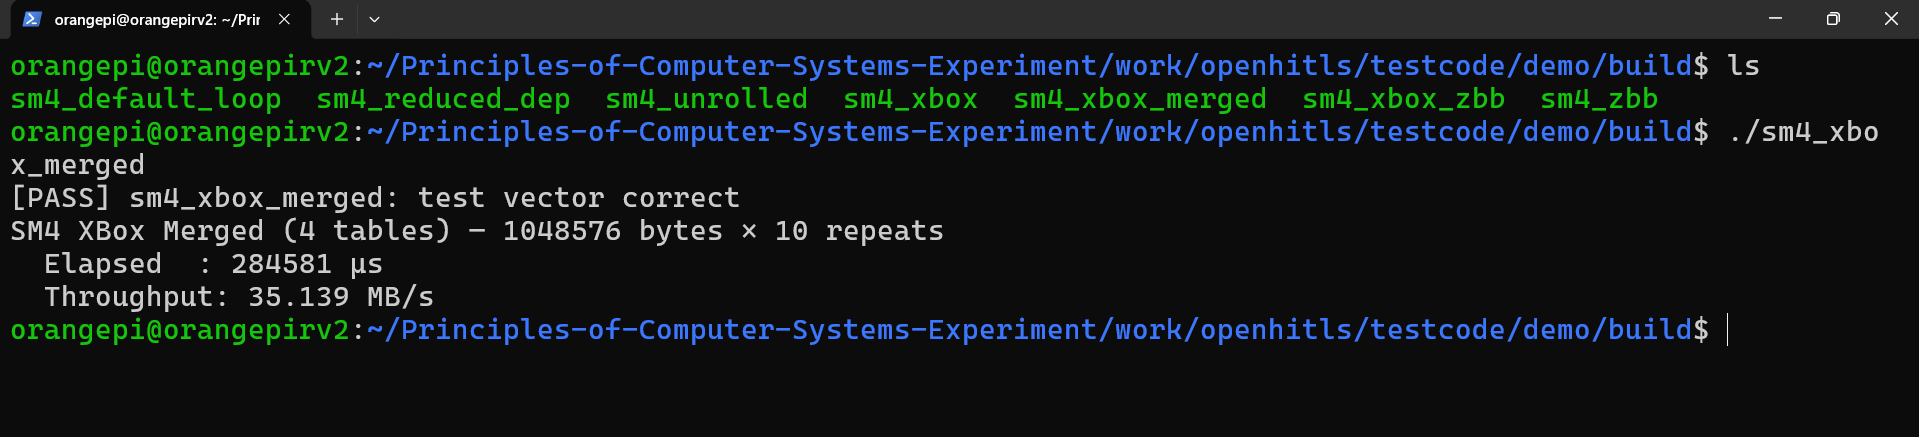
\includegraphics[width = 1\textwidth]{figure/sm4_xbox_merge}
    \caption{SM4XBox合并}
\end{figure}
可以看到程序运行效率和吞吐量相较之前版本优化得到很大提升,但因为需要预计算和存储4张表,因此有总计$4 * 256 * 4B = 4KB$的额外空间开销。
